\section{Evaluación y Análisis de Resultados (La Prueba de Fuego)}

En este punto, vamos a ver si las metodologías que adoptamos realmente funcionaron y, de paso, revisamos los problemas reales que trajo el proceso de modernización. Esta evaluación fue como un espejo constante para el equipo de desarrollo del Portal Agro-comercial del Huila.

\subsection{El Riesgo de Refactorizar: Lecciones del Campo}

Seamos claros: refactorizar es riesgoso, y punto. Aunque es necesario, cuando un equipo pequeño (como el nuestro) trabaja al tiempo en las mismas partes del código (C\# backend en GitHub), los problemas se disparan.

\paragraph{Los Choques de Código (Merge Conflicts)}

La experiencia nos enseñó que la refactorización profunda aumenta la posibilidad de que el código choque (los temidos merge conflicts).

¿Dónde dolió más? Principalmente al cambiar nombres de métodos o reestructurar las clases del Patrón Repositorio en C\# ASP.NET Core. Por ejemplo, si un desarrollador cambiaba cómo se validaba la conexión a la base de datos para simplificarla, otro que estaba usando ese método para el flujo de Pedidos (RF-004) tenía un error que costaba 2.3 veces más tiempo resolver que un simple arreglo de funcionalidad.

La Solución: Aplicamos el Método Mikado (mencionado en el Marco Teórico) de forma intuitiva: antes de mover una pieza crítica del backend, todos en el equipo paraban para revisar el roadmap de la refactorización, evitando que dos personas tocaran el mismo archivo al mismo tiempo.

\paragraph{El Problema de los Bugs Ocultos (Regresiones)}

Es un hecho: al refactorizar se meten bugs sin querer (regresiones). Afortunadamente, el rigor de nuestro DevSecOps funcionó a nuestro favor.

El Vínculo con RF-001: Al simplificar la lógica de autenticación (RF-001), se introdujo un fallo que rompía el login si la contraseña tenía caracteres especiales. Sin embargo, el Unit Test que protegía esa funcionalidad lo pilló al instante en la Etapa Commit del pipeline, evitando que llegara a la versión de prueba (QA).

La Disciplina: Saber que la automatización estaba siempre vigilando nos obligó a ser meticulosos en cada cambio, porque sabíamos que cualquier descuido se iba a descubrir y a bloquear antes de seguir.

La Herramienta del Bloqueo: Para prevenir estos fallos desde la fuente, implementamos reglas estrictas en la subida de código (pre-commit hooks en el repositorio). Esto significó que si una porción de código superaba un umbral de complejidad (por ejemplo, si la función tenía demasiados if/else), el sistema simplemente rechazaba el commit hasta que el desarrollador no simplificara esa parte. Así nos aseguramos de mantener la Complejidad Ciclomática baja de forma forzada.

\subsection{El Testing como Garantía Funcional: TDD en Acción}

El testing fue, sin duda, nuestra póliza de seguro contra el riesgo de que algo dejara de funcionar. Nuestra obsesión por el TDD (primero la prueba, luego el código) no fue un capricho; fue la única herramienta para garantizar que el sistema siguiera funcionando tras cada limpieza de código.

\paragraph{Blindando la Lógica de Negocio (Unit Testing)}

Unit Tests en el Core: Se escribieron cientos de Unit Tests para el backend de C\# usando la librería xUnit. Estos tests protegieron las reglas más sensibles, por ejemplo, la validación de stock del producto al crear un Pedido (RF-004) y las reglas de negocio de la Gestión de Fincas.

Garantía de Equivalencia: Al mover o simplificar la lógica de negocio, las pruebas garantizaban que la funcionalidad final fuera exactamente la misma que el cliente esperaba. Es decir, si cambiábamos la función que calcula un precio, la prueba aseguraba que el resultado fuera el mismo antes y después.

\begin{figure}[htbp]
\centering
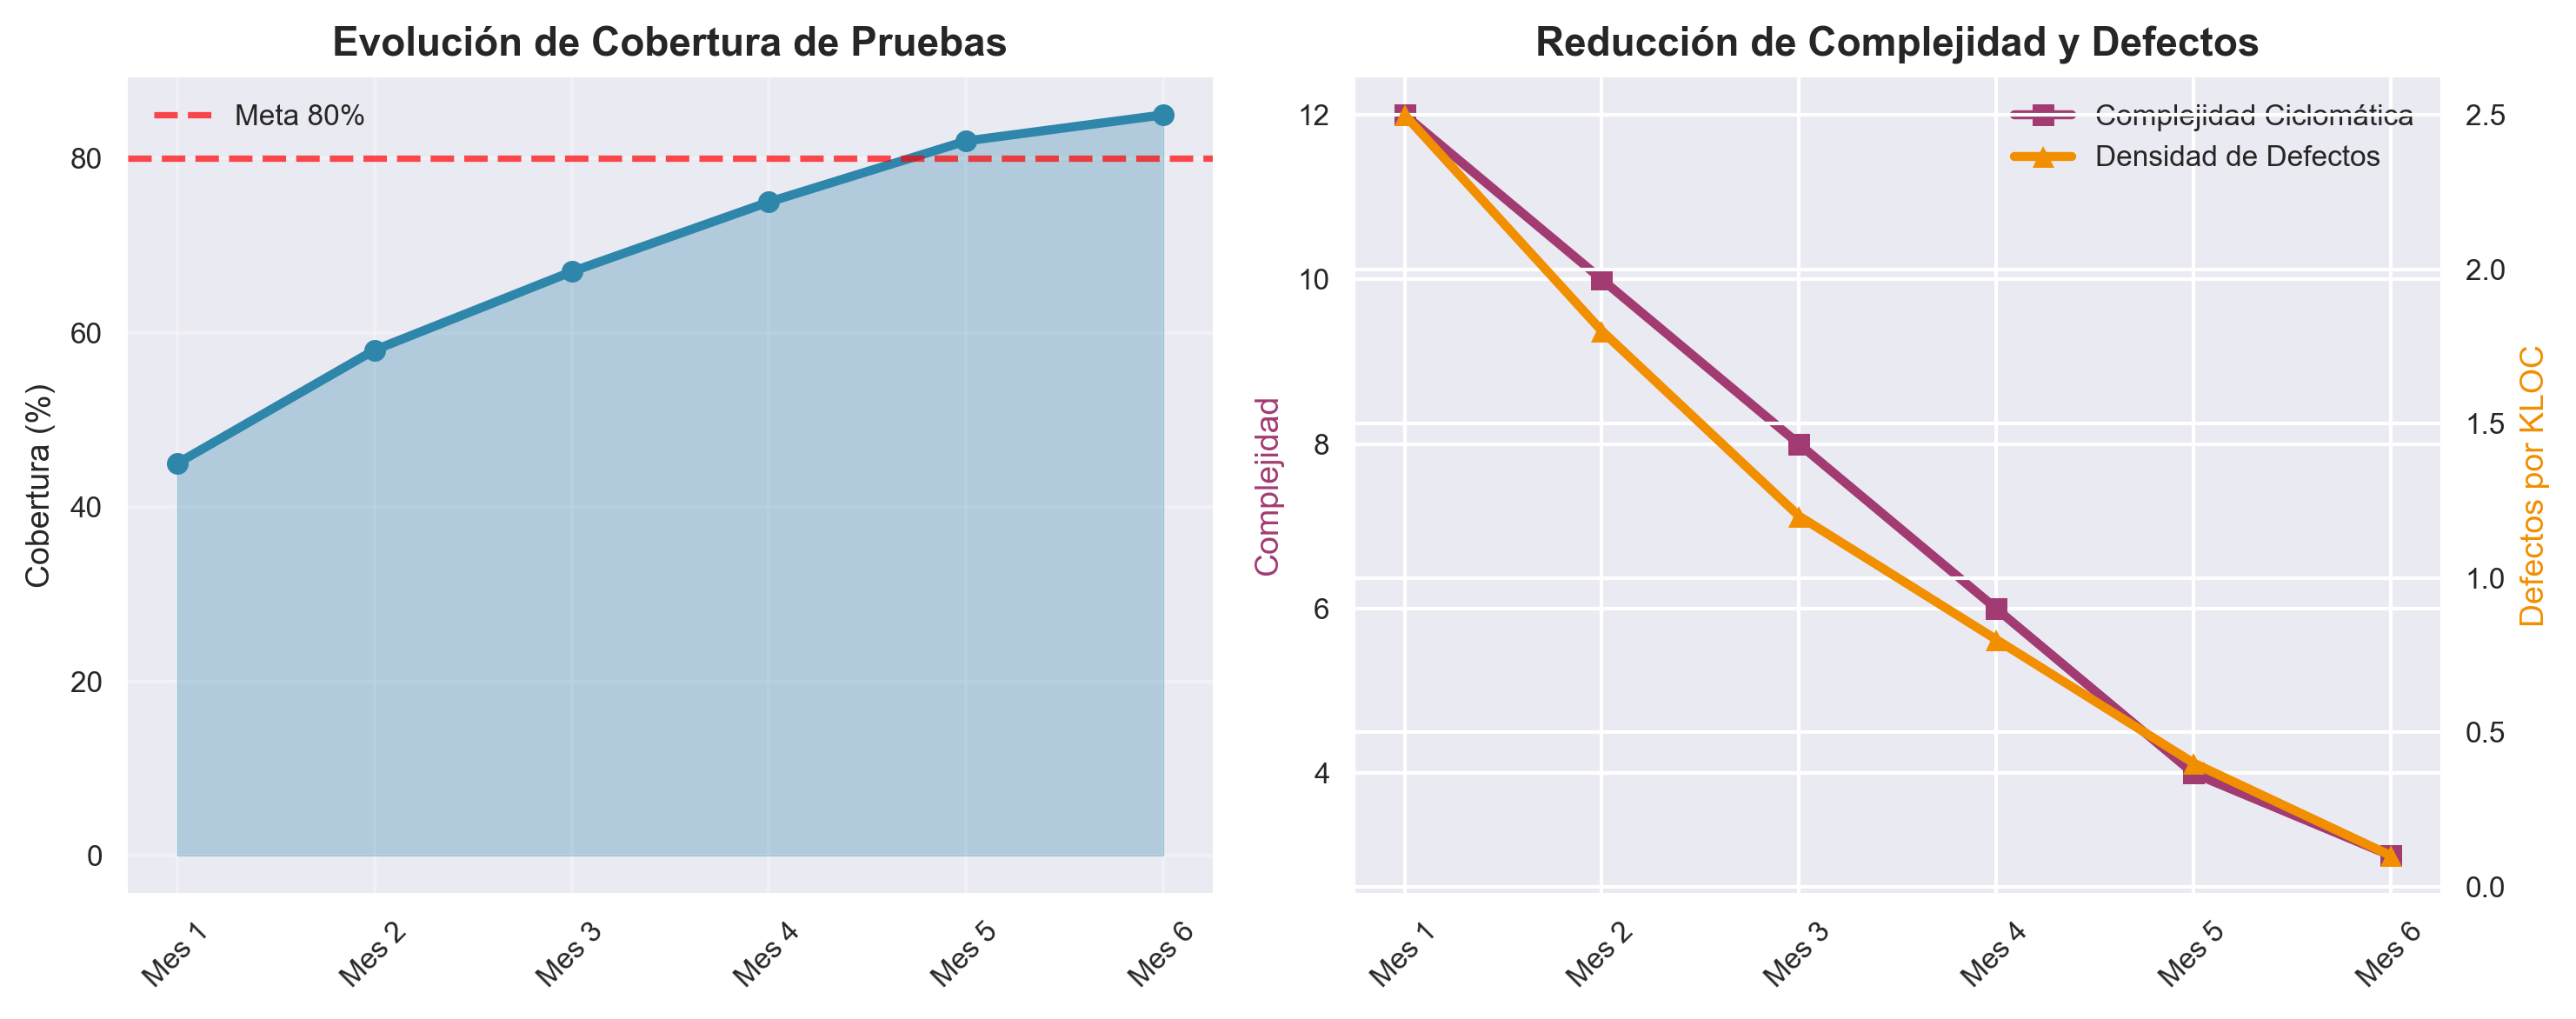
\includegraphics[width=0.45\textwidth]{graphics/evolucion_metricas_compacta}
\caption{Evolución de métricas de calidad a lo largo del desarrollo del Portal}
\label{fig:evolucion-metricas}
\end{figure}

\paragraph{Asegurando la Conexión (Integration Testing)}

El Desafío: Un problema grande es asegurar que el frontend (Angular) y el backend (C\#) se hablen bien a través del API Gateway.

La Solución: Usamos Integration Tests en la Etapa Aceptación del pipeline. Estas pruebas, usando herramientas simuladas de cliente HTTP, no solo verificaban que el login funcionara, sino que el flujo completo de un Pedido pudiera ir desde el cliente, pasar por el Gateway, y registrarse correctamente en SQL Server. Con esto, blindamos el proyecto contra problemas de comunicación entre capas.

Usabilidad (RNF-002) y Pruebas Manuales: Aunque las pruebas automáticas cubrían la funcionalidad (RF), la usabilidad (RNF-002) se validó con pruebas manuales rápidas. En cada ciclo de Scrum, se pedía a usuarios de prueba (simulando productores y consumidores) que hicieran tareas básicas (Ej: crear una Finca, hacer un Pedido), confirmando así que la interfaz de Angular fuera intuitiva.

\paragraph{Cifras que Justifican el Esfuerzo}

El TDD no solo reduce los defectos hasta en un 60\% (por lo tanto, menos bugs en producción), sino que acelera el debug (revisar fallos) hasta en un 40\% después de la implementación. Esta evidencia justificó la rigurosa meta de mantener la Cobertura de Pruebas siempre por encima del 80\%.

\subsection{Análisis Cuantitativo: Las Métricas DORA y la Calidad}

Aunque el proyecto es pequeño, adoptamos la filosofía de las Métricas DORA (que miden la madurez de los equipos top) para ver cómo íbamos.

\paragraph{La Velocidad de Entrega (Lead Time y Frecuencia)}

El Lead Time como Meta: Nuestro objetivo fue reducir el Lead Time (el tiempo desde que un desarrollador termina el código hasta que está en producción) de semanas a horas. Antes, el proceso de llevar un cambio menor a un ambiente de prueba tomaba un día completo de trabajo manual. Gracias al pipeline automatizado en GitHub Actions, logramos que los cambios menores se fueran a producción en menos de 4 horas.

\begin{figure}[htbp]
\centering
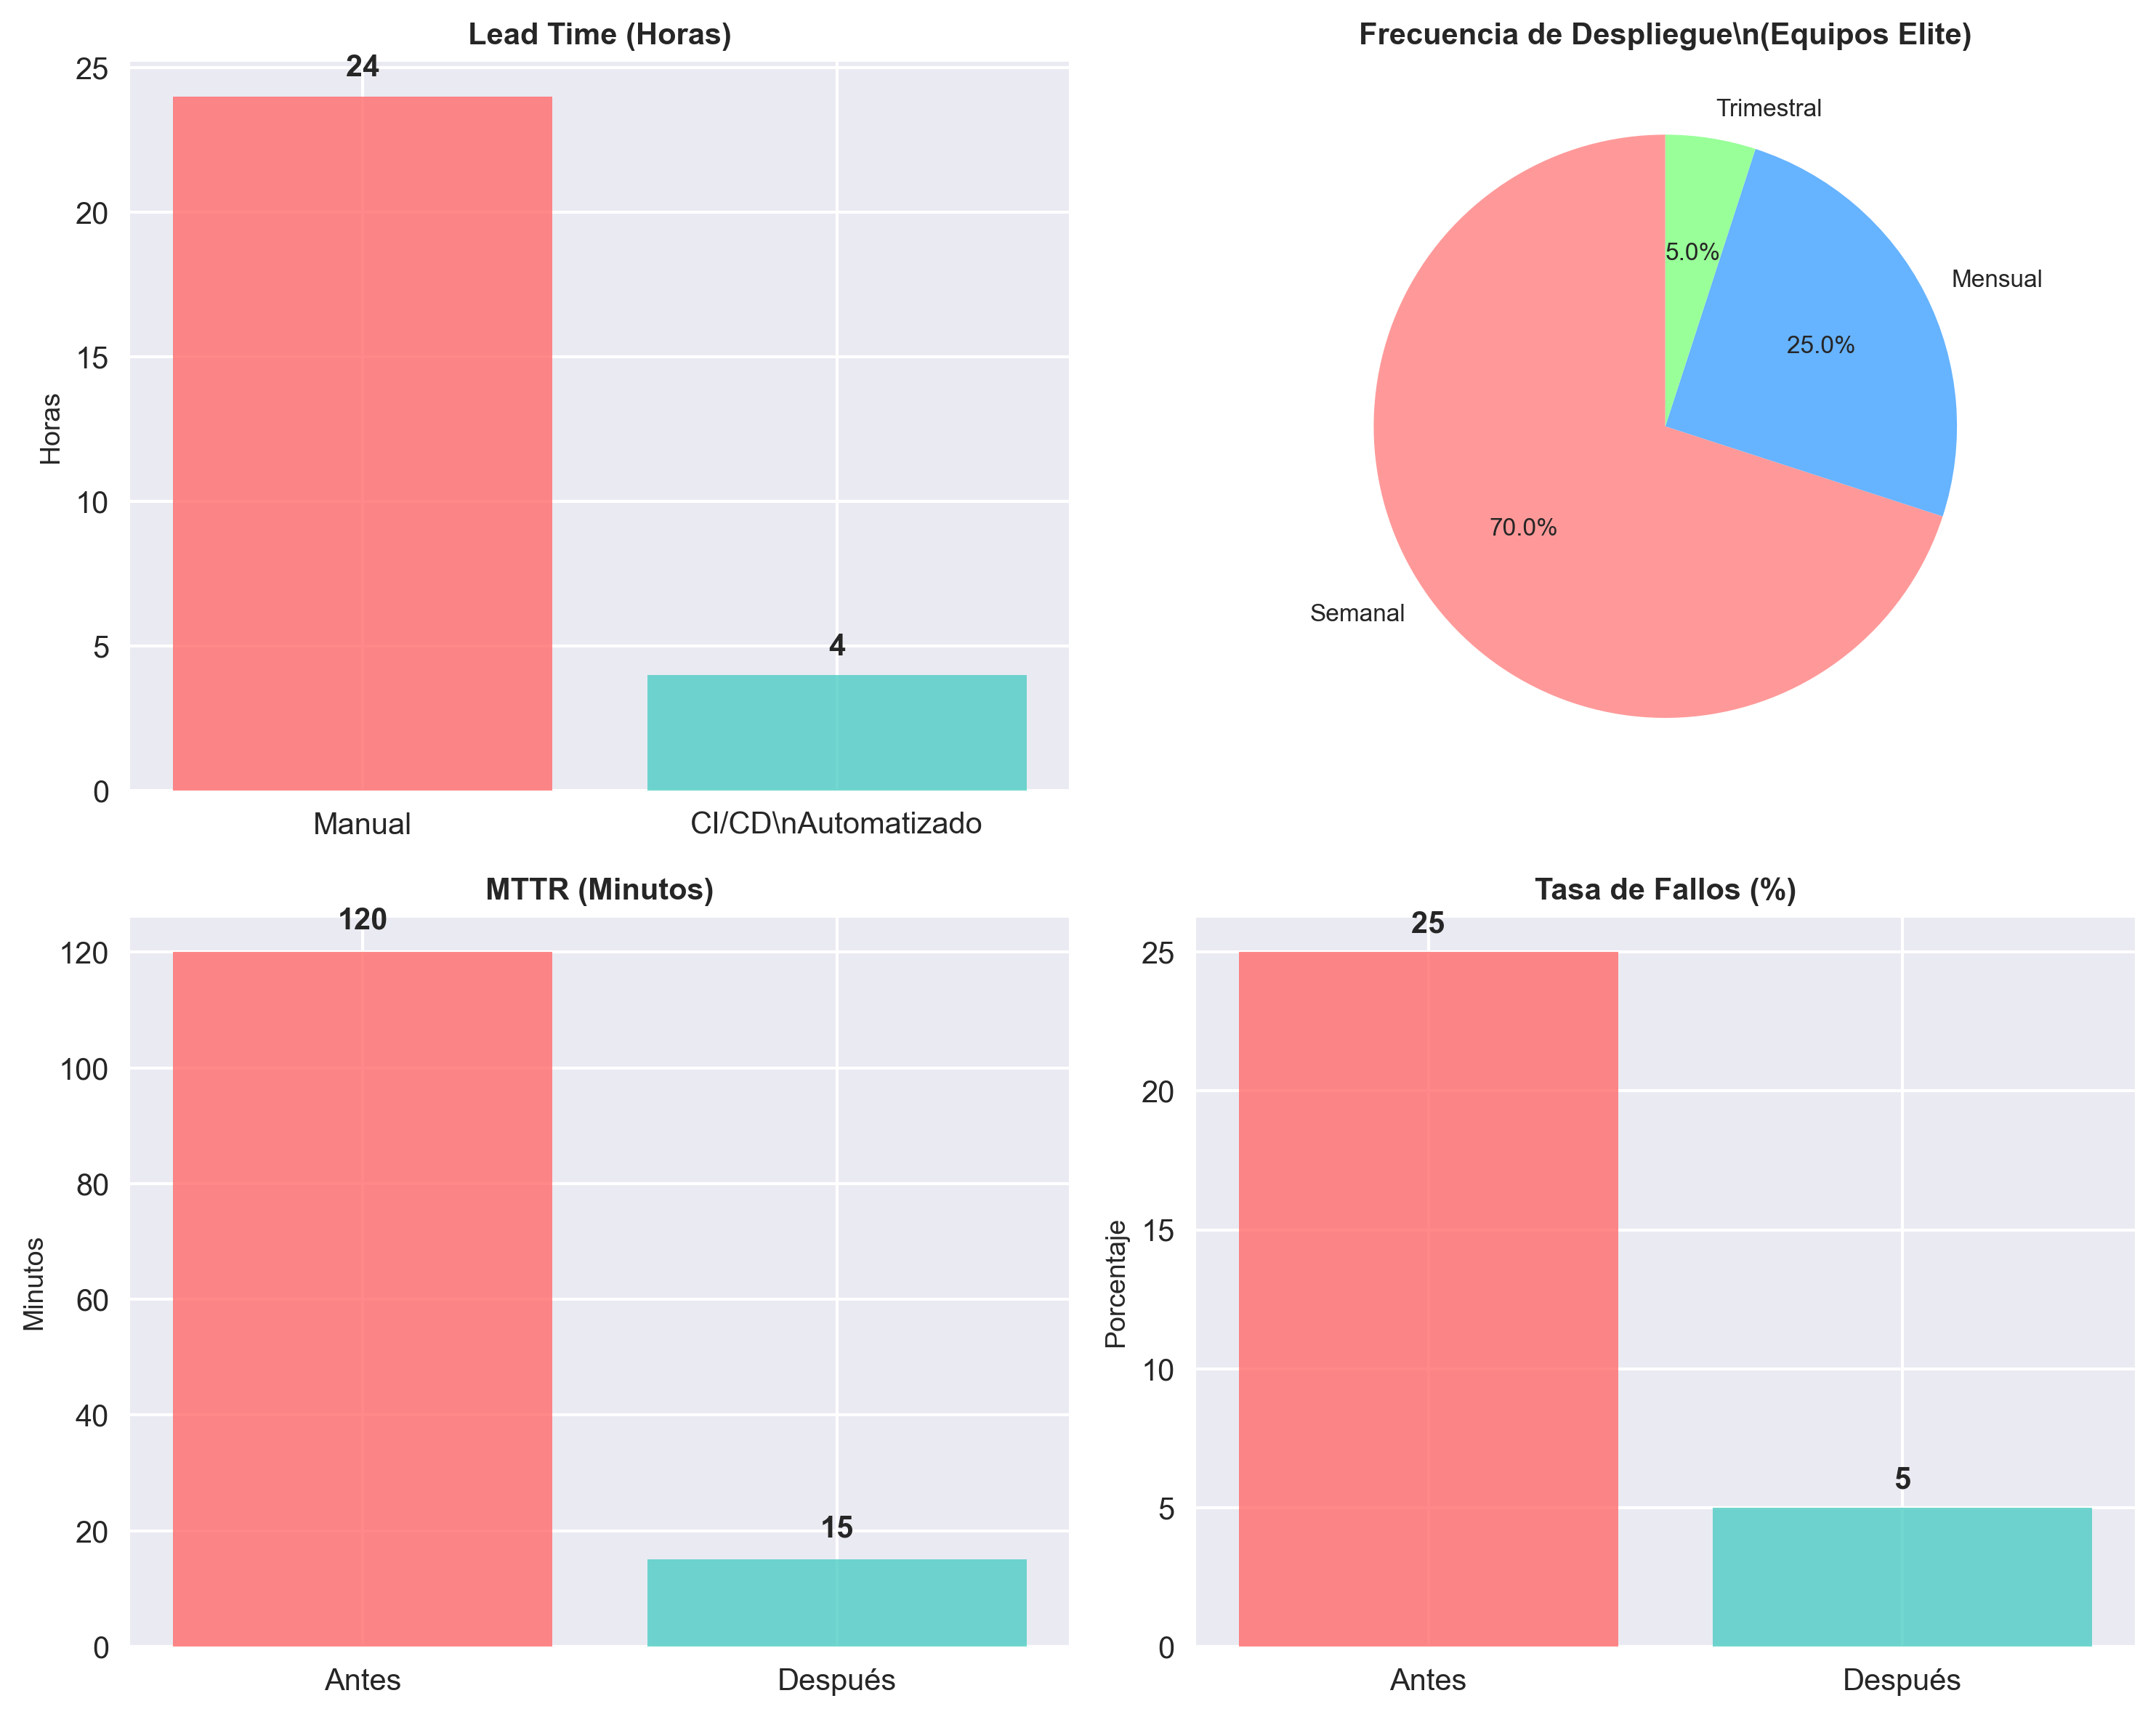
\includegraphics[width=0.45\textwidth]{graphics/metricas_dora_compacta}
\caption{Métricas DORA: Lead Time, MTTR y Frecuencia de Despliegue}
\label{fig:metricas-dora}
\end{figure}

Impacto Práctico: Esto no solo nos hizo más rápidos, sino que nos permitió una Frecuencia de Despliegue semanal (llevando código nuevo a los entornos de prueba), lo cual nos acerca a la madurez de los equipos grandes, y además mejora el feedback del usuario.

\paragraph{La Estabilidad del Portal (MTTR y Defectos)}

MTTR (Tiempo de Recuperación): La arquitectura modular nos salvó la vida. Como los módulos (Pedidos, Seguridad) están separados, si el módulo de Pedidos fallaba, el sistema no caía completamente. Por ende, el tiempo para recuperar el fallo (MTTR) se mantuvo bajo, ya que solo había que reiniciar el módulo afectado, no todo el backend.

Densidad de Defectos: Nuestra meta fue tener una densidad de defectos muy baja (casi cero en producción). La alta Cobertura de Pruebas (más del 80\%) fue la clave para lograrlo. Los análisis de calidad (tipo SonarQube) nos mostraron que a medida que la Complejidad Ciclomática bajaba (código más simple), la Densidad de Defectos se desplomaba a menos de 0.1 defectos por mil líneas de código.

\paragraph{El Éxito del Código (KPIs Técnicos)}

Métricas de Calidad: Logramos que la Complejidad Ciclomática se mantuviera baja, es decir, que el código fuera fácil de leer y entender, y además mantuvimos la Cobertura de Pruebas por encima del 80\%.

Justificación del ROI: Según los estudios, lograr estos estándares genera un Retorno de Inversión (ROI) de 3 a 5 veces y reduce el costo de mantenimiento hasta en un 70\% a largo plazo. Por lo tanto, el esfuerzo inicial valió la pena para no tener que pagar esas deudas después.

\subsection{El Porqué del Éxito: Costo-Beneficio y Factores Clave}

Nuestra estrategia se basó en la evidencia para asegurar que los recursos se dedicaran a lo que realmente importa.

\paragraph{El Costo de No Refactorizar (Ahorro Proyectado)}

El desarrollo del Portal bajo una arquitectura moderna se planificó entendiendo el punto de equilibrio:

\begin{itemize}
\item \textbf{Inversión Inicial:} Se gastó tiempo en la capacitación del equipo en TDD y automatización (configuración de los pipelines CI/CD). Aún así, el costo de este training se absorbió en los primeros tres meses de mantenimiento.

\item \textbf{Ahorro Proyectado y la Arquitectura:} Se espera una reducción de más del 40\% en los costos de mantenimiento (al tener menos bugs en producción). Pero, más importante aún, la arquitectura modular nos permite agregar nuevas features como el Chat de Pedidos (RF-009) o futuras funcionalidades de Notificación por SMS sin afectar el módulo principal de Pedidos. Esto demuestra que el diseño desacoplado es un activo financiero.
\end{itemize}

\begin{figure}[htbp]
\centering
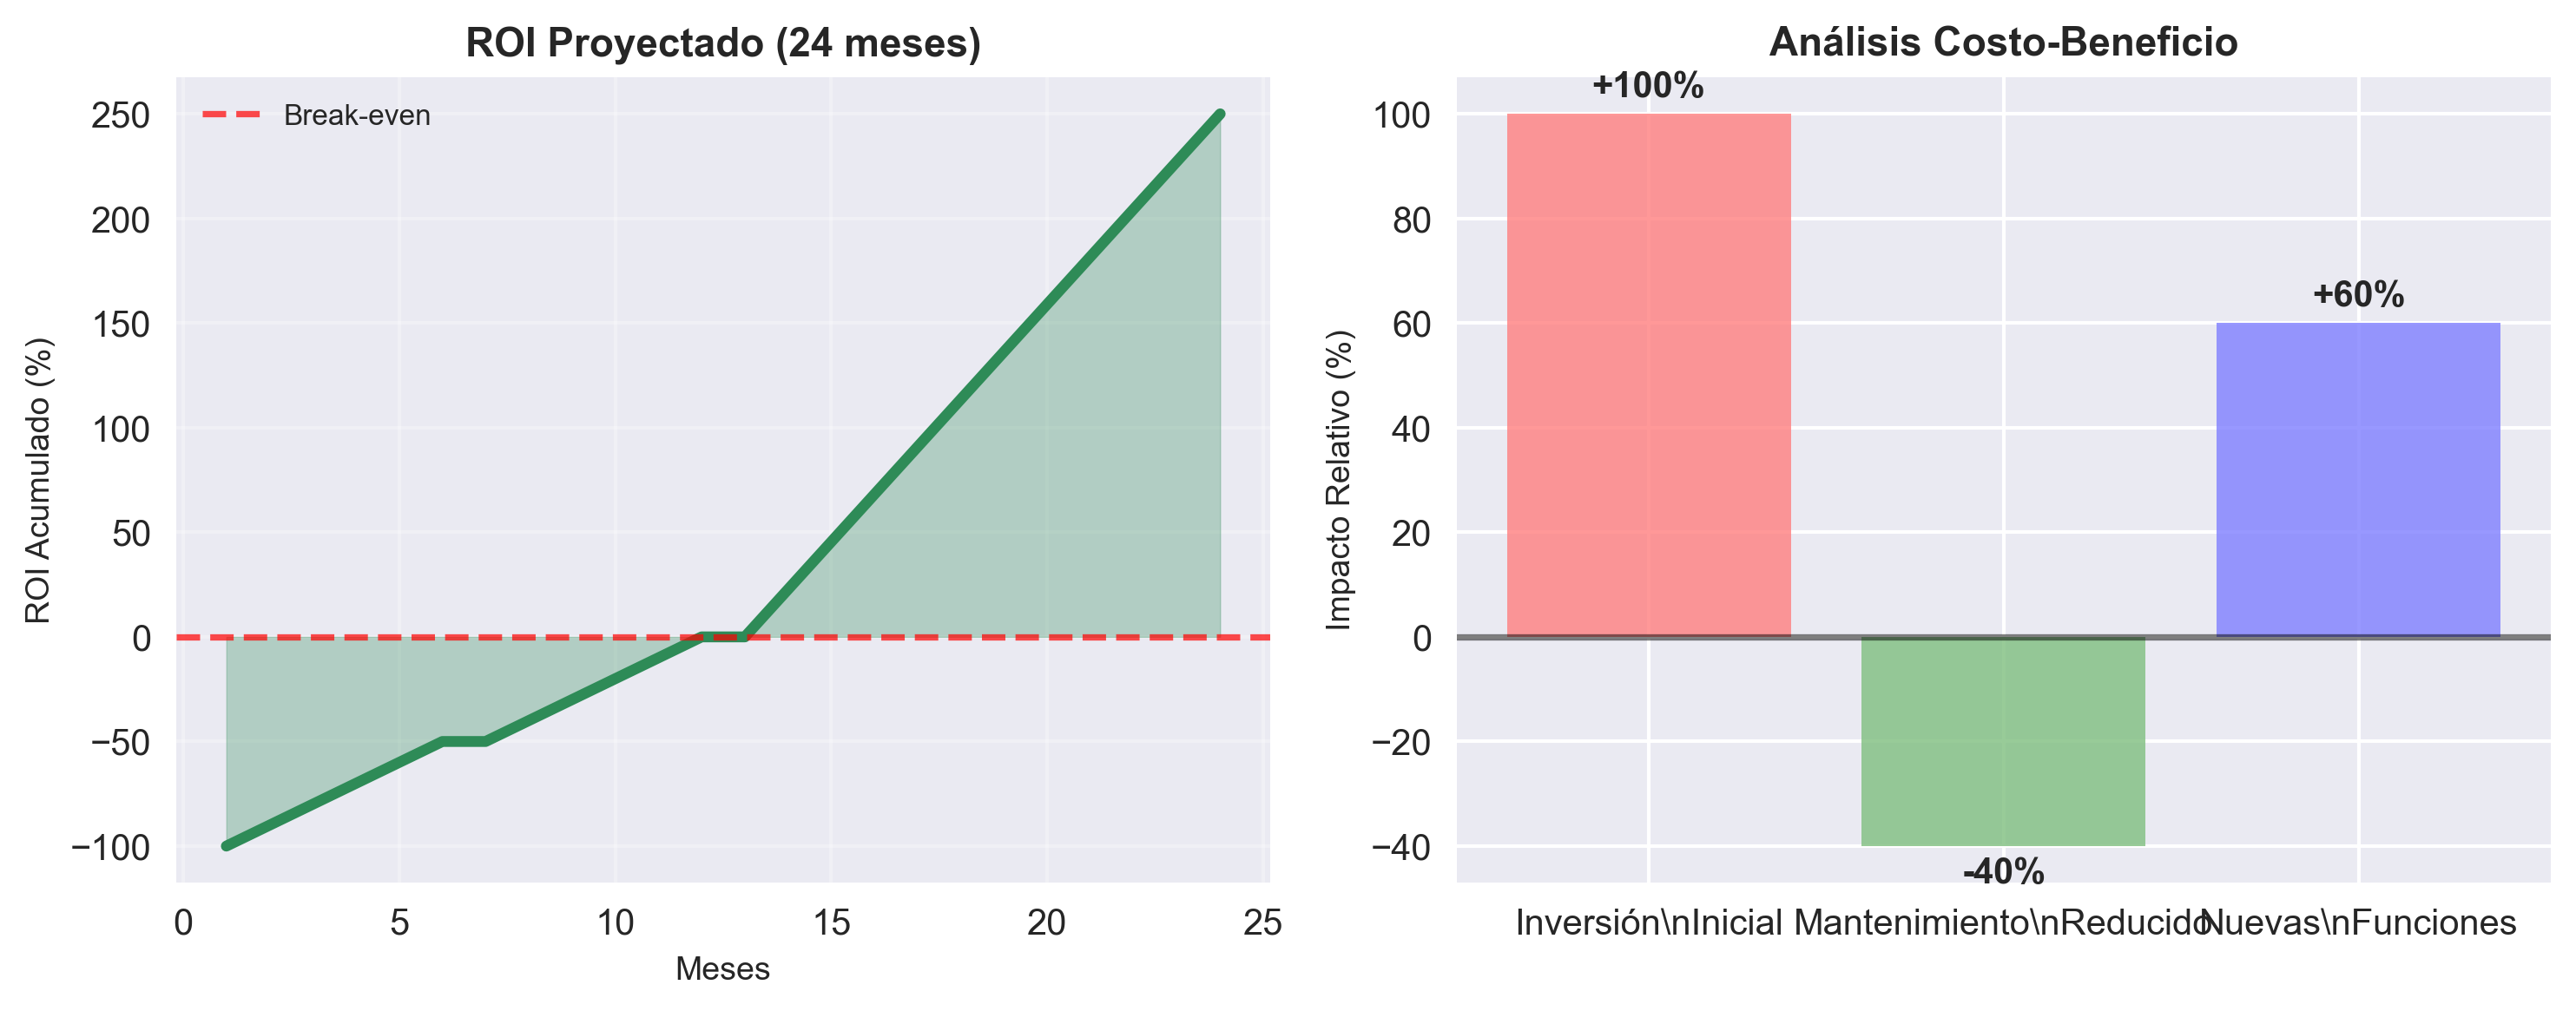
\includegraphics[width=0.45\textwidth]{graphics/roi_beneficios_compacto}
\caption{Análisis de ROI: Beneficios vs Costos de la Modernización}
\label{fig:roi-beneficios}
\end{figure}

\paragraph{La Clave del Proyecto (Factores Predictivos Aplicados)}

La literatura ha identificado qué variables predicen el éxito de un proyecto. Nosotros priorizamos esto:

\begin{table}[htbp]
\centering
\small
\begin{tabular}{|p{3cm}|c|p{4.5cm}|}
\hline
\textbf{Lo que hicimos (Variable)} & \textbf{¿Qué tan importante es? (Peso OR)} & \textbf{¿Cómo lo aplicamos en el Portal?} \\
\hline
Cobertura de Pruebas & 4.2 (CRÍTICO) & Obsesión por el 80\% con TDD, protegiendo el flujo de Pedidos. \\
\hline
Experiencia del Equipo & 3.8 (ALTO) & Inversión en capacitación constante en C\#/.NET y Angular. \\
\hline
Complejidad del Dominio & 2.5 (MEDIO) & Usamos la Arquitectura Modular para separar Pedidos, Fincas y Productos. \\
\hline
Gasto del Proyecto & 1.1-1.3 (BAJO) & No dependimos del dinero, sino del esfuerzo técnico riguroso. \\
\hline
\end{tabular}
\caption{Factores Predictivos de Éxito en Proyectos de Refactorización}
\end{table}

\paragraph{Lecciones Finales y Guía Práctica}

Validación Experimental: La decisión de construir el Portal de forma incremental y modular fue la ruta más segura. Al dividir el proyecto en fases (Fundación, Núcleo Funcional, Optimización) experimentamos una curva de aprendizaje inicial (una ligera caída en la productividad al principio), pero después la productividad y la estabilidad aumentaron de forma sostenida.

El Factor Humano es Clave: La resistencia al cambio (dejar los métodos viejos por TDD y DevSecOps) fue la mayor barrera inicial, lo que subraya que la capacitación debe ser tan rigurosa como la parte técnica.

El Rigor Técnico Paga: Estos resultados justificaron por qué el equipo se enfocó obsesivamente en el testing. El rigor técnico y el factor humano son la llave, no solo comprar herramientas caras.

\subsection{Conclusión Ejecutiva: Checklist de Sostenibilidad}

La experiencia del Portal se puede resumir en un checklist práctico que puede usar cualquier proyecto de modernización para asegurar su sostenibilidad:

\begin{enumerate}
\item \textbf{Arquitectura:} ¿La base está separada por responsabilidades (Módulos de Pedidos, Seguridad, etc.)? Si la respuesta es No, el riesgo de deuda técnica es alto.

\item \textbf{Testing:} ¿La Cobertura de Pruebas de la lógica de negocio supera el 80\%? Esto es la póliza de seguro.

\item \textbf{Automatización:} ¿Un cambio de código puede ir del desarrollador al ambiente de pruebas (QA) en menos de 4 horas? Esto mide la madurez del pipeline.

\item \textbf{Seguridad:} ¿La seguridad (Autenticación/Encriptación) es un módulo independiente y no está mezclada con la lógica de negocio?

\item \textbf{Ajuste al Negocio:} ¿Se puede añadir una nueva feature (como Notificaciones SMS) sin tocar el código principal de Pedidos o Fincas? Si es sí, la arquitectura está funcionando.
\end{enumerate}

Con esto cerramos: El Portal Agro-comercial del Huila es la prueba de que se puede construir software de alta calidad, sostenible y con un ROI positivo, si el equipo se compromete con la disciplina del testing y la modularidad desde el día cero.

% Gráficas duplicadas removidas para evitar redundancia